\section{Results}
\label{sec:results}

\subsection{Within-Model Convergence}
\label{sec:within}

\Tabref{tab:within} presents the within-model answer agreement rate (\aar) for each model--dataset combination under direct and CoT prompting. The central finding is that CoT's effect on convergence depends strongly on the task type.

\begin{table}[t]
\centering
\caption{Within-model answer agreement rate (\aar) under direct and CoT prompting. Higher \aar indicates more convergent outputs. We report mean $\pm$ standard deviation across 30 questions per dataset. Significant differences ($p < 0.05$, Wilcoxon signed-rank test) are marked with *.}
\label{tab:within}
\resizebox{\textwidth}{!}{%
\begin{tabular}{@{}llccccl@{}}
\toprule
\textbf{Model} & \textbf{Dataset} & \textbf{Direct \aar} & \textbf{CoT \aar} & \textbf{$\Delta$} & \textbf{Cohen's $d$} & \textbf{$p$-value} \\
\midrule
\multirow{3}{*}{\gptlarge}
& \gsm     & $0.870 \pm 0.275$ & $\mathbf{0.980 \pm 0.108}$ & $+0.110$ \increase & $+0.46$ & $0.027^*$ \\
& \csqa    & $\mathbf{0.980 \pm 0.108}$ & $0.733 \pm 0.275$ & $-0.247$ \decrease & $-0.91$ & $0.001^*$ \\
& \arc     & $\mathbf{1.000 \pm 0.000}$ & $0.871 \pm 0.228$ & $-0.129$ \decrease & $-0.56$ & $0.015^*$ \\
\midrule
\multirow{3}{*}{\gptmini}
& \gsm     & $0.753 \pm 0.320$ & $\mathbf{0.980 \pm 0.108}$ & $+0.227$ \increase & $+0.64$ & $0.006^*$ \\
& \csqa    & $\mathbf{0.947 \pm 0.171}$ & $0.927 \pm 0.197$ & $-0.020$ & $-0.11$ & $0.480$ \\
& \arc     & $\mathbf{0.964 \pm 0.132}$ & $0.904 \pm 0.213$ & $-0.061$ & $-0.23$ & $0.230$ \\
\midrule
\multirow{3}{*}{\gptnano}
& \gsm     & $0.560 \pm 0.377$ & $\mathbf{0.913 \pm 0.205}$ & $+0.353$ \increase & $+0.89$ & ${<}0.001^*$ \\
& \csqa    & $\mathbf{0.940 \pm 0.156}$ & $0.867 \pm 0.227$ & $-0.073$ & $-0.24$ & $0.169$ \\
& \arc     & $\mathbf{0.957 \pm 0.158}$ & $0.835 \pm 0.253$ & $-0.121$ & $-0.42$ & $0.070$ \\
\bottomrule
\end{tabular}
}
\end{table}

\para{Math: CoT increases convergence.} On \gsm, CoT significantly increases \aar for all three models ($p < 0.03$). The effect is strongest for the smallest model: \gptnano jumps from $0.560$ to $0.913$ ($d = +0.89$), while \gptlarge moves from $0.870$ to $0.980$ ($d = +0.46$). This pattern---larger effects for smaller models---suggests that CoT provides a computational scaffold that disproportionately benefits less capable models.

\para{Multiple-choice: CoT decreases convergence.} On \csqa and \arc, the trend reverses. \gptlarge shows significant decreases in \aar on both datasets, with a particularly large drop on \csqa (from $0.980$ to $0.733$, $d = -0.91$, $p = 0.001$). The smaller models show the same directional trend, though effects are smaller and not always significant. Under direct prompting, models achieve near-perfect \aar ($0.94$--$1.00$) on these multiple-choice tasks, suggesting that explicit reasoning introduces noise when models can already answer correctly by pattern matching.

\Figref{fig:within} visualizes the distribution of \aar values across questions, illustrating both the magnitude and consistency of these effects.

\begin{figure}[t]
\centering
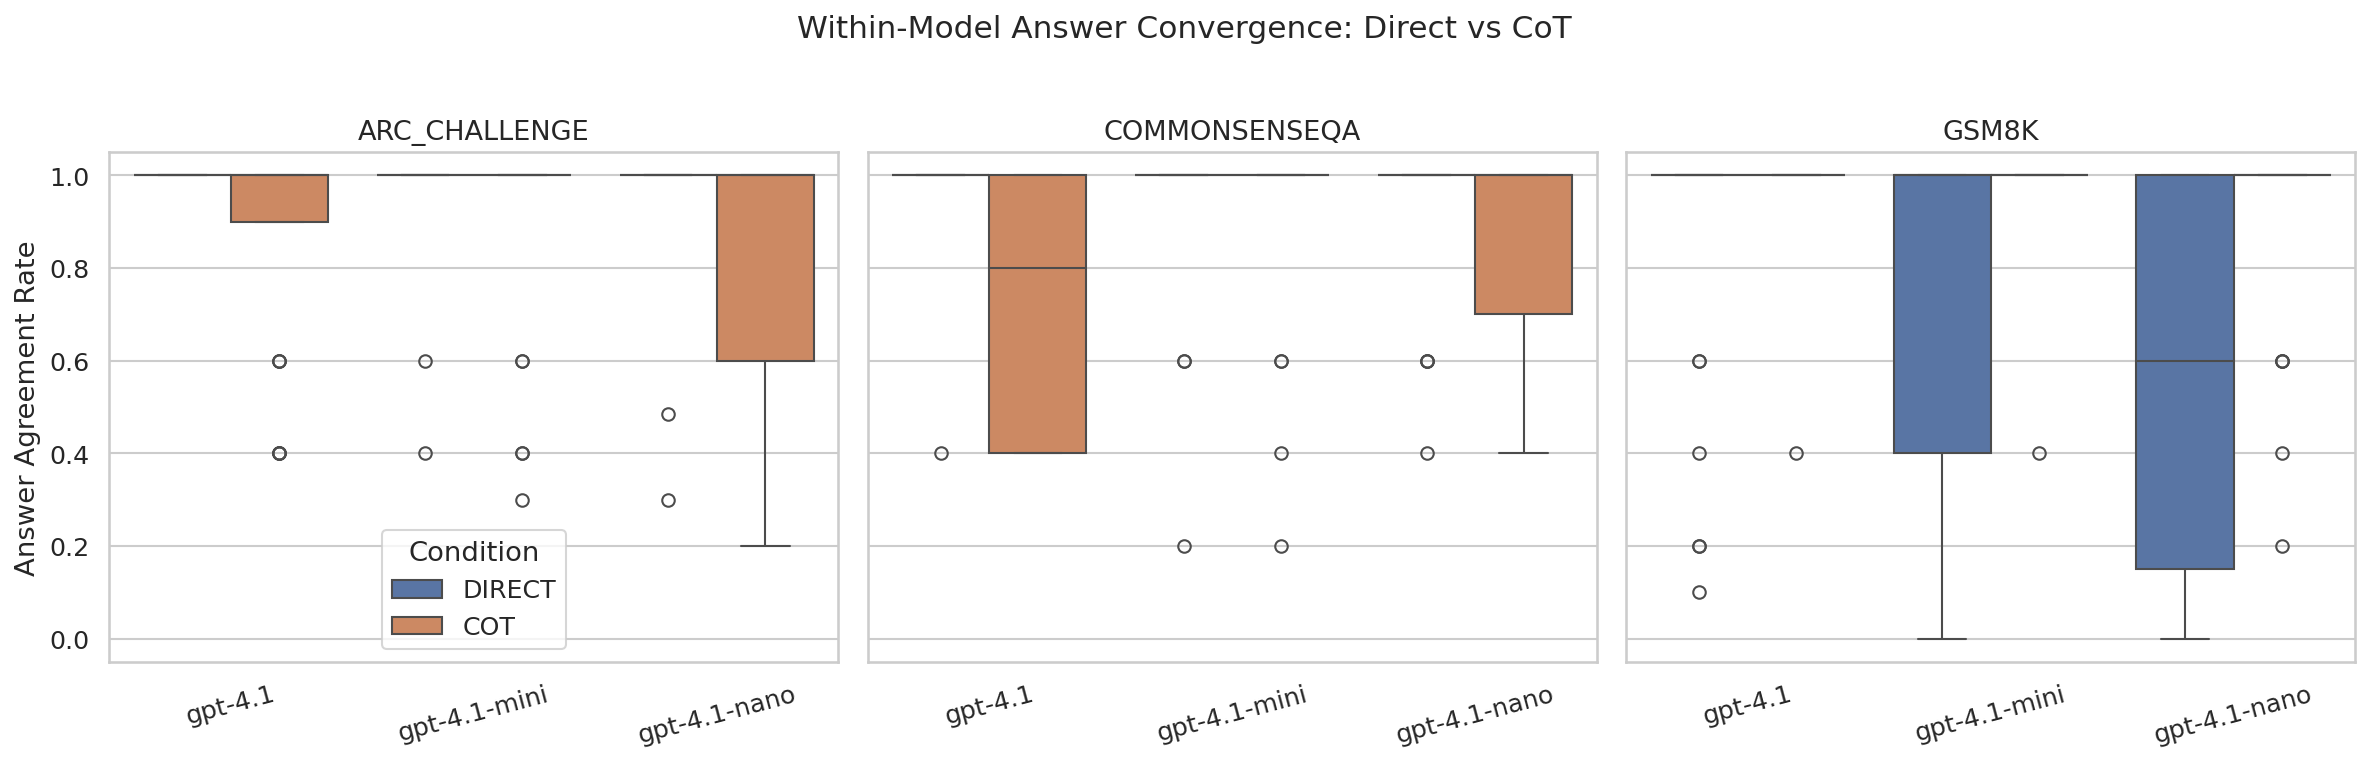
\includegraphics[width=0.95\linewidth]{figures/within_model_aar.png}
\caption{Distribution of within-model answer agreement rates (\aar) across 30 questions per dataset, comparing direct and CoT conditions. On \gsm (math), CoT shifts the distribution toward perfect agreement. On \csqa and \arc (multiple-choice), CoT spreads the distribution toward lower agreement. The effect is most pronounced for \gptlarge and \gptnano.}
\label{fig:within}
\end{figure}

\subsection{Cross-Model Convergence}
\label{sec:cross}

\Tabref{tab:cross} reports cross-model pairwise agreement for all model pairs. The same bidirectional pattern holds: CoT increases cross-model agreement on math but decreases it on multiple-choice tasks.

\begin{table}[t]
\centering
\caption{Cross-model pairwise agreement under direct and CoT prompting. Agreement is computed over all $5 \times 5 = 25$ sample pairs per question, averaged across 30 questions. Significant differences marked with *.}
\label{tab:cross}
\resizebox{\textwidth}{!}{%
\begin{tabular}{@{}llccccc@{}}
\toprule
\textbf{Model Pair} & \textbf{Dataset} & \textbf{Direct} & \textbf{CoT} & \textbf{$\Delta$} & \textbf{Cohen's $d$} & \textbf{$p$-value} \\
\midrule
\multirow{3}{*}{\gptlarge vs.\ \gptmini}
& \gsm     & $0.579$ & $\mathbf{0.984}$ & $+0.405$ \increase & $+0.96$ & ${<}0.001^*$ \\
& \csqa    & $\mathbf{0.940}$ & $0.739$ & $-0.201$ \decrease & $-0.74$ & ${<}0.001^*$ \\
& \arc     & $\mathbf{0.971}$ & $0.816$ & $-0.156$ \decrease & $-0.49$ & $0.022^*$ \\
\midrule
\multirow{3}{*}{\gptlarge vs.\ \gptnano}
& \gsm     & $0.212$ & $\mathbf{0.940}$ & $+0.728$ \increase & $+1.75$ & ${<}0.001^*$ \\
& \csqa    & $\mathbf{0.899}$ & $0.673$ & $-0.225$ \decrease & $-0.72$ & $0.002^*$ \\
& \arc     & $\mathbf{0.936}$ & $0.767$ & $-0.169$ \decrease & $-0.45$ & $0.021^*$ \\
\midrule
\multirow{3}{*}{\gptmini vs.\ \gptnano}
& \gsm     & $0.155$ & $\mathbf{0.940}$ & $+0.785$ \increase & $+2.39$ & ${<}0.001^*$ \\
& \csqa    & $\mathbf{0.889}$ & $0.843$ & $-0.047$ & $-0.17$ & $0.240$ \\
& \arc     & $\mathbf{0.907}$ & $0.843$ & $-0.064$ & $-0.21$ & $0.182$ \\
\bottomrule
\end{tabular}
}
\end{table}

\para{CoT bridges capability gaps on math.} The most striking result is the cross-model convergence on \gsm. Without CoT, \gptmini and \gptnano agree on only $15.5\%$ of math answers---barely above chance for open-ended numeric questions. With CoT, agreement jumps to $94.0\%$ (Cohen's $d = +2.39$, $p < 0.001$). Similarly, \gptlarge and \gptnano go from $21.2\%$ to $94.0\%$ agreement. CoT effectively erases the capability gap between models of vastly different sizes on mathematical reasoning.

\para{Cross-model divergence on multiple-choice.} On \csqa and \arc, CoT reduces cross-model agreement for pairs involving \gptlarge (the most affected model). The \gptlarge--\gptmini pair drops from $94.0\%$ to $73.9\%$ on \csqa ($d = -0.74$, $p < 0.001$). Pairs not involving \gptlarge show smaller, non-significant decreases, suggesting that the divergence effect is driven by the largest model's tendency to ``overthink'' on multiple-choice tasks.

\Figref{fig:cross} shows the distribution of cross-model agreement rates, highlighting the massive shift on \gsm and the moderate decrease on multiple-choice datasets.

\begin{figure}[t]
\centering
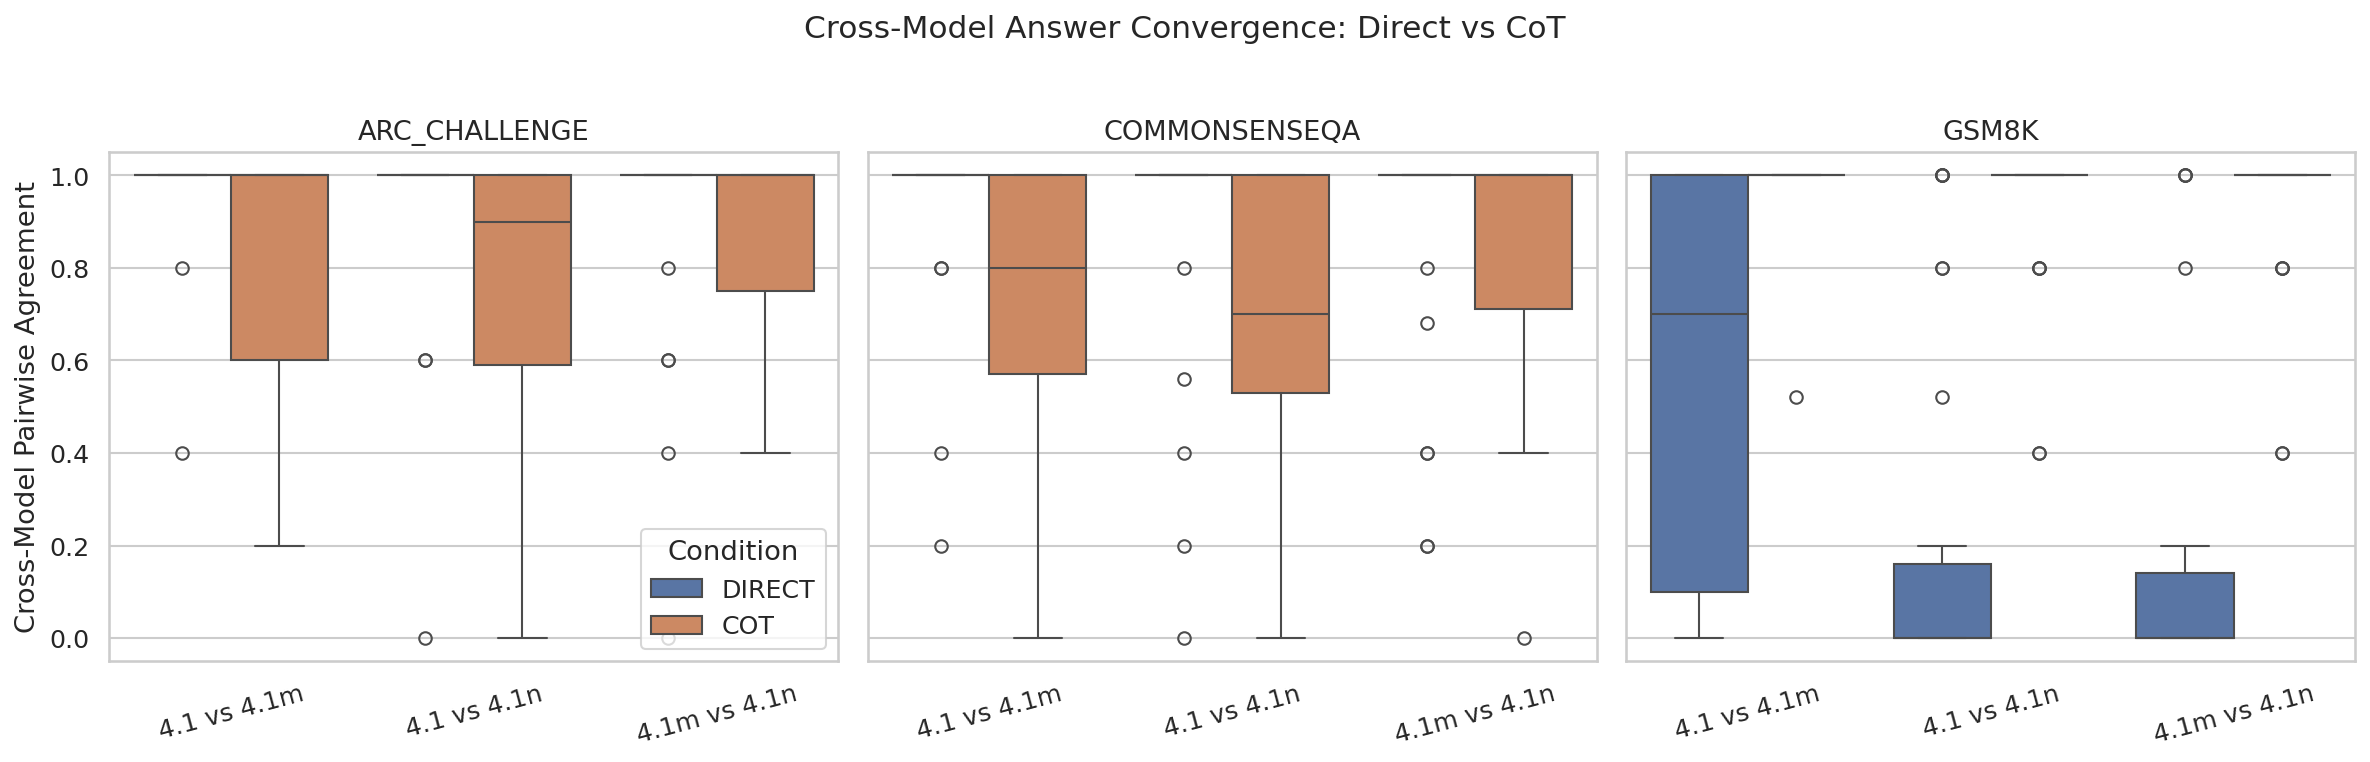
\includegraphics[width=0.95\linewidth]{figures/cross_model_agreement.png}
\caption{Distribution of cross-model pairwise agreement rates across 30 questions per dataset. On \gsm, CoT transforms near-random cross-model agreement into near-perfect agreement. On \csqa and \arc, CoT slightly reduces agreement, particularly for pairs involving the largest model.}
\label{fig:cross}
\end{figure}

\subsection{Accuracy and Convergence Are Coupled}
\label{sec:accuracy}

\Tabref{tab:accuracy} shows that the convergence pattern mirrors accuracy: where CoT increases accuracy, it also increases convergence, and vice versa.

\begin{table}[t]
\centering
\caption{Accuracy under direct and CoT prompting. CoT dramatically improves math accuracy (especially for smaller models) but slightly hurts multiple-choice accuracy, mirroring the convergence patterns in \tabref{tab:within} and \tabref{tab:cross}.}
\label{tab:accuracy}
\begin{tabular}{@{}llccc@{}}
\toprule
\textbf{Model} & \textbf{Dataset} & \textbf{Direct Acc.} & \textbf{CoT Acc.} & \textbf{$\Delta$} \\
\midrule
\multirow{3}{*}{\gptlarge}
& \gsm     & $0.700$ & $\mathbf{0.920}$ & $+0.220$ \increase \\
& \csqa    & $\mathbf{0.947}$ & $0.733$ & $-0.214$ \decrease \\
& \arc     & $\mathbf{0.929}$ & $0.864$ & $-0.065$ \decrease \\
\midrule
\multirow{3}{*}{\gptmini}
& \gsm     & $0.500$ & $\mathbf{0.920}$ & $+0.420$ \increase \\
& \csqa    & $\mathbf{0.927}$ & $0.920$ & $-0.007$ \\
& \arc     & $\mathbf{0.900}$ & $0.893$ & $-0.007$ \\
\midrule
\multirow{3}{*}{\gptnano}
& \gsm     & $0.187$ & $\mathbf{0.873}$ & $+0.686$ \increase \\
& \csqa    & $\mathbf{0.853}$ & $0.820$ & $-0.033$ \\
& \arc     & $\mathbf{0.864}$ & $0.821$ & $-0.043$ \\
\bottomrule
\end{tabular}
\end{table}

On \gsm, CoT improves accuracy by $+22.0$ to $+68.6$ percentage points, with the largest gains for \gptnano (from $18.7\%$ to $87.3\%$). Conversely, on \csqa, \gptlarge drops from $94.7\%$ to $73.3\%$---a substantial accuracy loss that parallels its convergence decrease. This coupling suggests that CoT-induced convergence is not an independent ``homogenization'' effect but rather a consequence of models converging toward correct answers: when CoT helps models find the right answer, they agree more; when it introduces reasoning errors, they diverge.

\subsection{Output Entropy}

\Figref{fig:entropy} confirms the convergence patterns through a complementary lens. On \gsm, CoT reduces output entropy (more convergent), while on \csqa and \arc, CoT increases entropy (more diverse).

\begin{figure}[t]
\centering
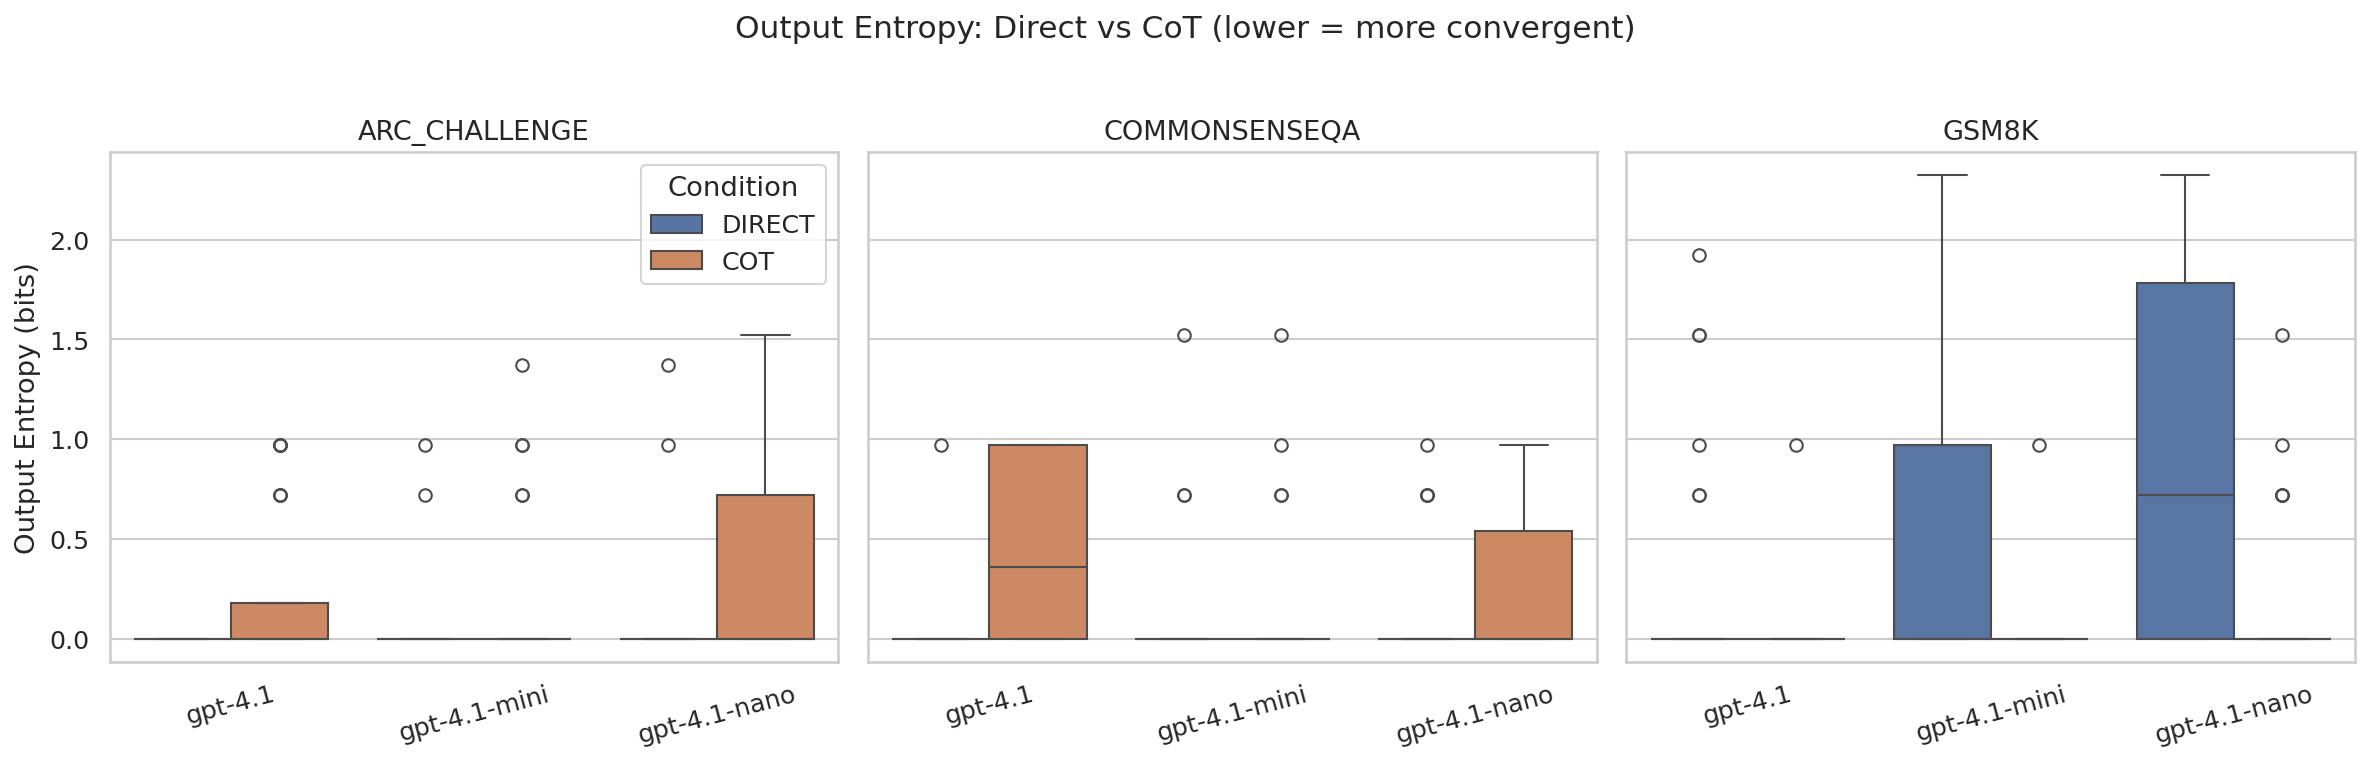
\includegraphics[width=0.95\linewidth]{figures/entropy_comparison.png}
\caption{Output entropy under direct and CoT conditions. Lower entropy indicates more convergent outputs. CoT reduces entropy on \gsm (math) while increasing entropy on \csqa and \arc (multiple-choice), consistent with the \aar results.}
\label{fig:entropy}
\end{figure}

For \gptlarge on \gsm, mean entropy drops from $0.246$ to $0.032$ with CoT. On \csqa, it rises from $0.032$ to $0.444$. The \gptnano pattern is even more dramatic: entropy drops from $0.880$ to $0.155$ on math but rises from $0.105$ to $0.226$ on commonsense. These entropy measurements, being a different operationalization of convergence than \aar, provide converging evidence for the bidirectional effect.

\subsection{Summary of Hypothesis Tests}

\Tabref{tab:hypotheses} summarizes the status of our four hypotheses.

\begin{table}[h]
\centering
\caption{Summary of hypothesis testing outcomes.}
\label{tab:hypotheses}
\begin{tabular}{@{}lll@{}}
\toprule
\textbf{Hypothesis} & \textbf{Result} & \textbf{Key Evidence} \\
\midrule
H1: CoT $\uparrow$ within-model convergence & Partially supported & Math: $p < 0.03$; MC: reversed \\
H2: CoT $\uparrow$ cross-model convergence & Partially supported & Math: $d$ up to $+2.39$; MC: reversed \\
H3: CoT $\uparrow$ response similarity & Not tested & Answer-level only \\
H4: Stronger effect on structured tasks & Strongly supported & Math $d > 0$, MC $d < 0$ \\
\bottomrule
\end{tabular}
\end{table}
